\chapter{Implementation}
% how the different tools speak to communicate and the main roles of each tool, in broad terms
The tool has now been used in a practical example to give an idea of how it is used to enhance the development experience.
This chapter will go into the design decisions and implementation details to make each part and feature of the tool function, as well as,
explain what the tool consists of and how the components work together to create the finished product.

\section{Overview of the Components}
The tool essentially consists of four components: The VS Code extension, the Svelte user interface, the Java program, and the NodeJS utility program.
The Java program is used to run the Jolie parser, which is also written in Java, and that will gather all information from the Jolie code needed by the visualization tool.

The Svelte user interface is the component which takes in the user input and renders the services, ports and connections.
In order for the UI to get the relevant data from the Jolie code, the VS Code extension invokes the NodeJS utility program, with the correct parameters, which invokes the Java program. 
The NodeJS program listens for the output of the Java program,
meaning that the NodeJS program functions as a wrapper for the Java tool so the VS Code extension does not have to invoke the Java tool directly,
and sends the data to the VS Code extension, which sends the data to the Svelte UI.

Figure \ref*{figure:init_tool_sequence} shows the process of initializing the tool in VS Code, which is done using the \textit{visualize} command in VS Code.

\clearpage
\section{Data Representation}

\begin{figure}[t]
    \center
    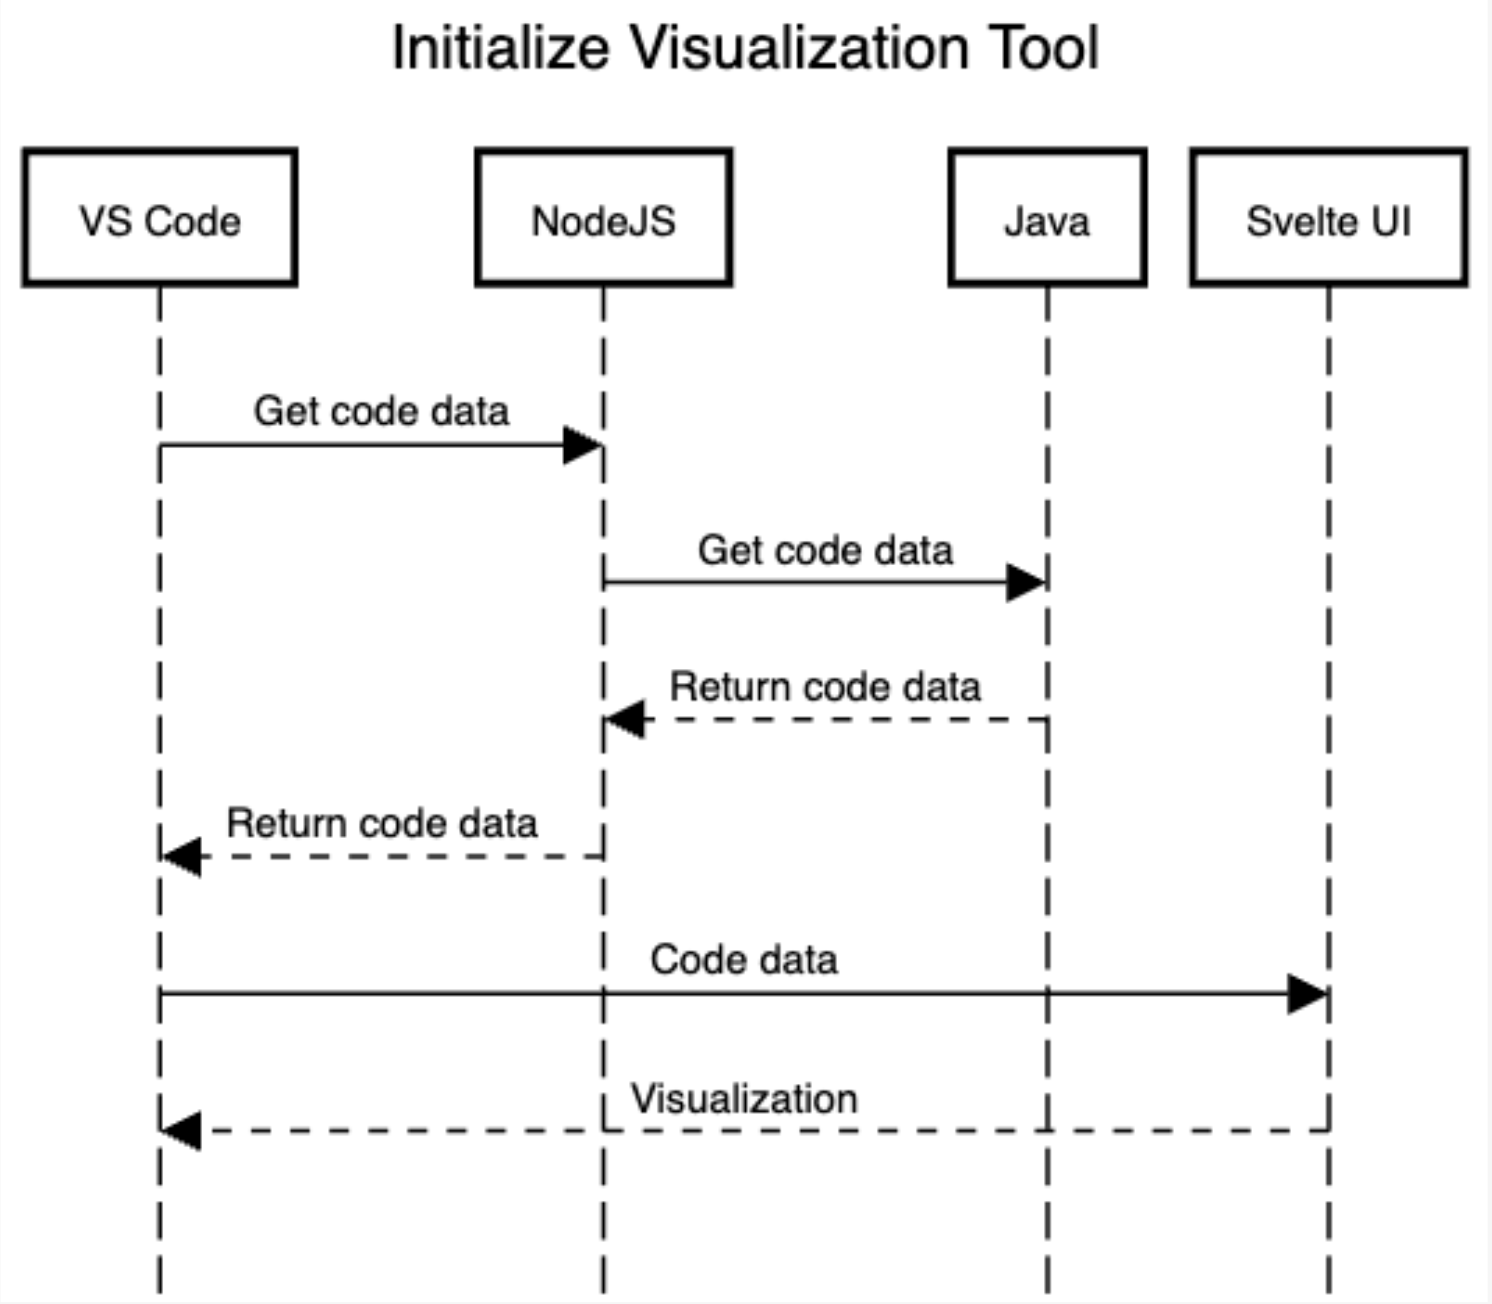
\includegraphics[width=0.70\textwidth]{figures/init_tool_sequence.png}
    \caption{A sequence diagram showing the sequence of requests and invocations between the four components that the tool consists of. The VS Code extension invokes the utility program using NodeJS which will handle running the Java program with the correct parameters, and afterwards, the VS Code extension sends that data to the Svelte UI which will visualize it in VS Code.}
    \label{figure:init_tool_sequence}
\end{figure}

The data which the Java program will output has to be consistent through all
four components of the tool. The chosen data format is JSON data because it is easy to parse in TypeScript, which all components consist of except for the Java program.

% how the data is represented from the Jolie parser
% bigraph inspiration

\section{Java Program}
% how the data is fetched in the Java tool

\section{Visualization User Interface}
% what is the problem. requirements.
\subsection{UI Library}
% discussion
% svelte
\subsection{Rendering}
% discussion
% elk


\section{Visual Studio Code Extension}
% how the vscode extension works
% vscode api
% webviews
% live reload

\section{NodeJS Utility Program}
% why it is created and how it works

\section{Refactoring}
\subsection{Code Refactoring}
% Editing properties of the services and ports using the sidebar
\subsection{Embedding \& Disembedding}
% auto import
\subsection{The Aggregator Pattern}

\section{Prototyping}
% generating docker compose files
% getting dependencies